% This work is licensed under the Creative Commons
% Attribution-NonCommercial 3.0 Unported License. To view a copy of this
% license, visit http://creativecommons.org/licenses/by-nc/3.0/.

\section{Durchführung}
\subsection{Zur Signalbearbeitung}
Es werden nach und nach Bauteile des Lock-In-Verstärkers hinzugeschaltet und daraufhin mithilfe eines Oszilloskops das Ausgangssignal betrachtet. In Abb. \ref{fig:aufbau} ist eine schematische Darstellung der einzelnen Bauteile des Lock-In-Verstärkers zu sehen.
\subsubsection{Nicht verrauschtes Signal}
Als erstes wird ein sinusförmiges Signal mit einer Spannungsamplitude von \SI{20}{\milli\volt} und einer Frequenz von \SI{1}{\kilo\hertz} vom eingebauten Funktionsgenerator erzeugt. Ein Bild dieses Signals ist in Abb. \ref{fig:anfangssignal_ohne_rausch} zu finden. Außerdem liefert der Funktionsgenerator ein weiteres Sinussignal, das sog. Referenzsignal, welches beim Mischer benötigt wird. Das Referenzsignal besitzt eine nicht veränderbare Spannungsamplitude von \SI{3.2}{\volt} und ebenfalls eine Frequenz von ca. \SI{1}{\kilo\hertz}. Eine Abbildung des Referenzsignals ist in Abb. \ref{fig:referenzsignal_ohne_rausch} zu sehen.
Anschließend wird das zu messende Signal durch den Verstärker verstärkt.
Im nächsten Schritt wird das verstärkte Signal im Mischer mit dem Referenzsignal multipliziert. Dabei kommt es, je nach Phasenunterschied, zu unterschiedlichen Ergebnissen. In diesem Versuch werden die Ergebnisse für fünf verschiedene Phasen untersucht, welche sich in den Abbildungen \ref{fig:phase_0_nicht_verrauscht} bis \ref{fig:phase_270_nicht_verrauscht} wiederfinden. Die angegebene Phase bezeichnet hierbei nicht den Phasenunterschied zwischen zu bearbeitendem Signal und Referenzsignal, sondern den Wert, um welchem der Phasenschieber das Referenzsignal verschiebt.
Zuletzt wird das gemischte Signal auf einen Tiefpass gegeben. Das dabei entstehende Signal ist eine Gleichspannung, welche je nach eingestellter Phasenverschiebung einen anderen Spannungswert besitzt (siehe Theorie). Es werden zu 10 verschiedenen Phasen die Spannungswerte der entstehenden Gleichspannung am Oszilloskop gemessen. Ein Bild von einer dieser Gleichspannungen ist in Abb. \ref{fig:gleichspannung_ohne_rausch} zu sehen.

\begin{figure}
\centering
\label{fig:aufbau}
\includegraphics{aufbau.pdf}
\caption{Schematische Darstellung der Bauteile des Lock-In-Verstärkers}
\end{figure}

\subsubsection{Verrauschtes Signal}
Nun wird im wesentlichen der gesamte oben genannte Vorgang wiederholt, allerdings mit einem verrauschten Sinussignal, anstatt eines reinen Sinussignals. Dazu wird das bereits vom Funktionsgenerator vorhandene Sinussignal mittels Rauschgenerator verrauscht. Das unmittelbare Ergebnis dieses Verrauschens ist in Abb. \ref{fig:vollrausch} abgebildet. Das verrauschte Signal wird zunächst wieder im Verstärker verstärkt. Dieses Signal wird mittels Bandpassfilter von Frequenzen befreit, die sich stark von der zu messenden Frequenz von etwa \SI{1}{\kilo\hertz} unterscheiden. Das Signal hat dannach die in Abb. \ref{fig:bandrausch} wiedergegebene Form. Anschließend wird das verrauschte Signal im Mischer mit demselben Referenzsignal wie im vorherigen Abschnitt gemischt. Dabei kommt es wieder, je nach Phasengang, zu unterschiedlichen Ergebnissen. Auch hier wurden die entstehenden Signale bei fünf verschiedenen Phasen betrachtet. Diese sind in den Abbildungen \ref{fig:phase_0_verrauscht} bis \ref{fig:phase_270_verrauscht} zu finden.
Im letzten Schritt wird das gemischte Signal auf einen Tiefpass gegeben. Von der dabei entstehenden Gleichspannung werden wieder 10 Messwerte in Abhängigkeit von der eingestellten Phasenverschiebung aufgenommen.

\subsection{Zur Messung der Lichtintensität}
Mithilfe des Lock-In-Verstärkers wird nun eine Messreihe gestartet, in der die Lichtintensität in Abhängigkeit des Abstandes zur Lichtquelle gemessen wird. Dazu wird eine Leuchtdiode mit einer vom Funktionsgenerator generierten Rechteckspannung mit maximal einstellbarer Amplitude betrieben. Mit einer Photodiode wird die Lichtintensität gemessen. Dazu werden die in der Leuchtdiode entstehenden Spannungen als Eingangssignal in den Lock-In-Verstärker gegeben. Der Bandpassfilter wird so eingestellt, dass die Amplituden des Signals nach dem Bandpass maximal werden. Der Phasenschieber verschiebt die Phase des Referenzsignals ebenfalls genau so, dass die Amplituden des Ausgangssignals maximal werden. Als Endergebnis erhält man wieder eine Gleichspannung, welche Proportional zur Spannung der Photodiode ist, welche wiederum proportional zur Lichtintensität bei der Photodiode ist. Es wird nun eine Messreihe gestartet, in der der Spannungswert der Gleichspannung am Ausgang des Lock-In-Verstärkers in Abhängigkeit des Abstandes zwischen Leuchtdiode und Photodiode gemessen wird. Um auch noch bei größeren Entfernungen messen zu können, wird der Faktor, mit dem der Verstärker das Signal verstärkt während des Versuches immer wieder erhöht. Dieser Gain-Wert muss bei der Auswertung der Messergebnisse berücksichtigt werden.